\documentclass[10pt,letterpaper]{article}
\usepackage[margin=0.75in]{geometry}
\usepackage{amsmath,amssymb,array,booktabs,tabularx}
\usepackage[shortlabels]{enumitem}
\usepackage[dvipsnames]{xcolor}
\usepackage{fancyhdr}
\usepackage{tikz}
\setlength{\parindent}{0pt}
\setlength{\parskip}{0.35em}
\renewcommand{\arraystretch}{1.15}
\newcolumntype{Y}{>{\raggedright\arraybackslash}X}
\newcommand{\spacefor}[1]{\vspace{#1}}
\newcommand{\blank}{\rule{0.75cm}{0.4pt}}
\pagestyle{fancy}
\fancyhf{}
\lhead{MA371: Project 1 ASDS/CS Inquiry}
\rhead{AY27-1}
\cfoot{\thepage}
\setlength{\headheight}{14pt}

\begin{document}
\begin{center}
{\Large\bfseries One Link, Many Paths: A PageRank Decision}\\[3pt]
{\large Guided inquiry packet: Applied Data Science and Computer Science}
\end{center}
\textbf{Name:} \rule{2.4in}{0.4pt}\hfill
\textbf{Inquiry partners:} \rule{2.25in}{0.4pt}

\textbf{Decision brief.} The director of a fictional predeployment training portal can add exactly \emph{one} navigation link to a Reference Card (R). The choice is a link from the Home page (H) or a link from the Planning Guide (P). Which edit, if either, should the director make to improve the card's discoverability? Substantiate your advice with a link-network model and explain what evidence would be needed before claiming that actual cadets will find or use the card more often. All pages, links, and click records in this packet are \textbf{synthetic teaching data}; no real military system or personnel are represented.



\textbf{Relevant MA371 connections.} Lesson 17: eigenvalues and eigenvectors. Lesson 18: eigenvector modes and diagonalization \emph{when a matrix is diagonalizable}. Lesson 19: discrete dynamical systems and interpretation of a model in context. The directed graph, PageRank, and validation ideas are introduced here; no coding or characteristic polynomial of a $5\times5$ matrix is required.

\textbf{Suggested class rhythm (50 minutes).} 8 minutes: learn the directed-link rule; 12: build the five-page matrix; 10: interpret iteration and eigen-information; 10: compare edits; 7: challenge the model with clicks and sensitivity; 3: frame a claim. Complete the memo and annex after class.

\section*{1. Learn the directed-link rule on three pages}
An arrow $j\to i$ means that \emph{page $j$ contains a link to page $i$}. A directed link need not have a reverse link. For pages A, B, and C, suppose A links to B and C, B links to C, and C links to A and B:
\[
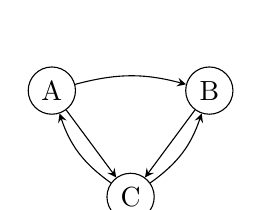
\begin{tikzpicture}[baseline=-0.5ex,>=stealth,every node/.style={circle,draw,minimum size=6mm,inner sep=0pt}]
\node (a) at (0,0) {A}; \node (b) at (2,0) {B}; \node (c) at (1,-1.35) {C};
\draw[->] (a) to[bend left=15] (b);
\draw[->] (a) -- (c);
\draw[->] (b) -- (c);
\draw[->] (c) to[bend left=18] (a);
\draw[->] (c) to[bend right=18] (b);
\end{tikzpicture}
\qquad
T_{\rm ex}=\begin{bmatrix}
0&0&1/2\\ 1/2&0&1/2\\ 1/2&1&0
\end{bmatrix}.
\]
Here \textbf{origin pages are columns} and destination pages are rows. A visitor following a link chooses uniformly among the links on the current page. Thus $T_{ij}$ is the modeled chance of following a link from origin $j$ to destination $i$. Check the arrows against every column. Each column sums to $1$.

\begin{enumerate}[a.,leftmargin=*]
\item Why is $T_{\rm ex}$ not symmetric? Explain the entries $T_{\mathrm{B},\mathrm{A}}=1/2$ and $T_{\mathrm{C},\mathrm{B}}=1$ in words.\\[0.36in]
\item A visitor is certainly on page A, represented by $\vec p_0=(1,0,0)^T$. Compute $T_{\rm ex}\vec p_0$ and interpret each coordinate.\\[0.36in]
\end{enumerate}

\newpage
\section*{2. From a page list to a transition matrix}
The portal has five pages in the fixed order below. A \emph{link} just means a visible navigation hyperlink, not necessarily evidence of a click, page quality, or endorsement.
\begin{center}
\begin{tabularx}{\linewidth}{@{}p{0.48in}p{1.55in}Y@{}}
\toprule
Label & Page & Existing outgoing links\\
\midrule
H & Home & P, S, E\\
P & Planning Guide & H, E\\
S & Safety Checklist & H, E\\
E & Worked Examples & P, R\\
R & Reference Card & H\\
\bottomrule
\end{tabularx}
\end{center}
\textbf{Proposals.} Option 1 adds H$\to$R; Option 2 adds P$\to$R. All other links remain unchanged. Exactly one proposal may be selected. In this baseline network every page has at least one outgoing link.

First construct a binary \textbf{adjacency matrix} $A$: $A_{ij}=1$ if origin page $j$ links to destination page $i$, and $0$ otherwise. Let $d_j$ be the number of outgoing links from page $j$. Next construct the \textbf{link-following matrix} $T$ by dividing each nonzero entry in column $j$ by $d_j$: $T_{ij}=A_{ij}/d_j$. The order of the rows and columns is H, P, S, E, R.

\begin{enumerate}[a.,leftmargin=*]
\item Draw five labeled vertices and all directed arrows in the baseline network. Circle the two arrows that are \emph{proposed but not yet present}.\\[0.90in]
\item Fill the baseline adjacency matrix. Why should the H column contain three $1$s? Why need $A$ not be symmetric?
\[
A=\begin{bmatrix}
\blank&\blank&\blank&\blank&\blank\\
\blank&\blank&\blank&\blank&\blank\\
\blank&\blank&\blank&\blank&\blank\\
\blank&\blank&\blank&\blank&\blank\\
\blank&\blank&\blank&\blank&\blank
\end{bmatrix}
\quad\begin{matrix} \mathrm H\\\mathrm P\\\mathrm S\\\mathrm E\\\mathrm R\end{matrix}
\]
\item Give the outgoing-link counts $(d_{\rm H},d_{\rm P},d_{\rm S},d_{\rm E},d_{\rm R})$. Construct the H, P, and R columns of $T$; state why \emph{every} column sums to $1$.\\[0.72in]
\item Under Option 1, which single column of $T$ changes? Give the new probability of following H$\to$P and H$\to$R. Repeat for P$\to$H and P$\to$R under Option 2.\\[0.58in]
\end{enumerate}

\textbf{A missing-link edge case.} If a page has no outgoing links, its raw $A$ column is zero and cannot be normalized by $d_j$. Our stated rule is to replace that \emph{dangling page's} link-following column by the uniform vector $\vec u=(1/5)\vec 1$. This is a modeling convention, not a claim that a visitor actually clicks a nonexistent link. What would go wrong with the total probability if the zero column were left unchanged?\\

\newpage
\section*{3. Why PageRank is a discrete dynamical system}
A visitor does not always click a link. In our \textbf{random-surfer model}, each step follows an outgoing link with probability $\alpha=0.85$ and otherwise restarts uniformly on one of the five pages. Define
\[
G=\alpha T+(1-\alpha)\vec u\vec 1^{\,T},\qquad
\vec u=\tfrac15\vec 1,\qquad
\underbrace{\vec p_{k+1}}_{5\times1}=\underbrace{G}_{5\times5}\underbrace{\vec p_k}_{5\times1}.
\]
The coordinate $(\vec p_k)_i$ is the modeled share of visits on page $i$ after $k$ navigation steps. The update is \emph{discrete} (one step at a time), \emph{dynamic} (the distribution changes), and \emph{linear} (matrix multiplication forms the next distribution). We assume the same links and click rule at every step. This is a modeled probability distribution, not a guarantee about a particular cadet or a validated forecast of real behavior.

\textbf{Worked bridge on the three-page example.} There, use $\alpha=0.85$ and $\vec u=(1/3,1/3,1/3)^T$. Starting on A, a link is followed with probability $0.85$ and a uniform restart puts $0.05$ on each page. Therefore
\[
G_{\rm ex}(1,0,0)^T=(0.05,0.475,0.475)^T.
\]
The two $0.475$ entries each consist of $0.85(1/2)+0.05$. This one-step distribution is \emph{not} the long-run ranking.

\begin{enumerate}[a.,leftmargin=*]
\item Verify the C column of $G_{\rm ex}$ using the arrows. Explain why every column of $G$ sums to $1$ and has positive entries.\\[0.48in]
\item For the five-page baseline, start with $\vec p_0=\vec u=(0.2,0.2,0.2,0.2,0.2)^T$. Calculate $(\vec p_1)_{\rm R}$ by hand. Identify the link-following contribution and the restart contribution.\\[0.52in]
\item Without computing a characteristic polynomial, explain why $\vec p_k=G^k\vec p_0$. What does a fixed vector $\vec p_*$ satisfying $G\vec p_*=\vec p_*$ represent? Which eigenvalue belongs to it, and why must it be normalized so $\vec 1^{\,T}\vec p_*=1$?\\[0.67in]
\end{enumerate}

With uniform restart and $0<\alpha<1$, this $G$ has strictly positive entries. The model therefore has one positive stationary probability vector, and iteration from any starting distribution approaches it. If $G$ also has an eigenvector basis, we know that $G$ is diagonalizable, hence have the expression $G^k=PD^kP^{-1}$ that describes how nonstationary modes fade. \emph{Do not assume every directed-link matrix is diagonalizable.} You do not need its full eigendecomposition to interpret the stationary vector.

\textbf{Computation check.} A later calculator can iterate $\vec p_{k+1}=G\vec p_k$ until successive vectors are sufficiently close. A useful numerical check is $\|G\vec p_*-\vec p_*\|_1$ together with $\vec 1^{\,T}\vec p_*=1$. What do these checks establish, and what do they \emph{not} establish about real user behavior?\\[0.44in]

\newpage
\section*{4. Compare the two link edits before recommending one}
The following are supplied \textbf{machine-computed model results} for uniform restart and $\alpha=0.85$. They are rounded to four decimals. The computation used the exact link list, not these rounded values. Use them to interpret and audit a result, not as a substitute for constructing $A$ and $T$.
\begin{center}
\begin{tabular}{@{}lrrrrr@{}}
\toprule
Network & $p_{*,\rm H}$ & $p_{*,\rm P}$ & $p_{*,\rm S}$ & $p_{*,\rm E}$ & $p_{*,\rm R}$\\
\midrule
Baseline & .2853 & .2172 & .1108 & .2503 & .1364\\
Option 1: H$\to$R & .3108 & .1882 & .0960 & .2168 & .1882\\
Option 2: P$\to$R & .2880 & .2037 & .1116 & .2168 & .1799\\
\bottomrule
\end{tabular}
\end{center}
Under the \emph{stated criterion}, a larger $p_{*,\rm R}$ is better: it is the Reference Card's long-run share in this modeled navigation process. It is \emph{not} a measured fraction of cadets who found the card or learned its contents.

\begin{enumerate}[a.,leftmargin=*]
\item \textbf{Predict before consulting the numbers:} Which origin page seems more promising for the new link? Explain why the origin's modeled visibility and its number of outgoing links may both matter.\\[0.43in]
\item Calculate the increase in $p_{*,\rm R}$ over baseline for each option, in \emph{percentage points}. How far apart are the two options? Do not label that difference a percent increase without specifying the denominator.\\[0.54in]
\item Does the highest-ranked page necessarily contain the most valuable or most frequently used content? Explain why a rank ordering alone cannot settle the director's decision.\\[0.47in]
\item The card R links back to H. Notice that Option 1 changes H's own stationary share as well as R's. Why can a link edit affect pages other than its destination? Use the idea of repeated navigation rather than a single click.\\[0.55in]
\end{enumerate}

\textbf{Interrogate the algorithm.} A common implementation error treats outgoing links as rows but still multiplies a \emph{column} vector on the right. State one check that would detect this orientation error. Then explain why a tiny stationary residual would \emph{not} reveal that the original link list was wrong.\\[0.58in]

\newpage

\section*{5. Test assumptions with held-out click observations}
The following \emph{synthetic held-out} records were not used to construct $T$. Each row summarizes 100 page-to-page clicks that \emph{started} on its listed origin, pooled over time. These are 300 click events, not necessarily 300 distinct cadets. The records describe the \emph{baseline} site, before either proposed link exists.
\begin{center}
\begin{tabular}{@{}lrrrrr@{}}
\toprule
Origin $\backslash$ destination & H & P & S & E & R\\
\midrule
H & 0 & 52 & 33 & 15 & 0\\
P & 70 & 0 & 0 & 30 & 0\\
E & 0 & 25 & 0 & 0 & 75\\
\bottomrule
\end{tabular}
\end{center}
\begin{enumerate}[a.,leftmargin=*]
\item Normalize the H row of counts to write an empirical \emph{H column} of click probabilities in destination order H, P, S, E, R. Compare it with the model's equal-link H column. Which destination has the largest absolute discrepancy?\\[0.56in]
\item What aspect of the baseline model do these observations challenge? Why can they \emph{not} directly validate the effect of either new link?\\[0.49in]
\item If you wanted a click-weighted transition matrix for the entire baseline portal, which additional origin-page records would you need? What would remain unknown about the proposed links?\\[0.46in]
\end{enumerate}
\newpage
\section*{6. Stress-test the claim and write the memo}
The continuation probability $\alpha$ expresses how often the modeled visitor follows a link rather than restarts. Compare the following sensitivity results, again using \emph{uniform} restart and the same exact link lists:
\begin{center}
\begin{tabular}{@{}lrrr@{}}
\toprule
$\alpha$ & Baseline $p_{*,\rm R}$ & Option 1 $p_{*,\rm R}$ & Option 2 $p_{*,\rm R}$\\
\midrule
$0.65$ & .1478 & .1876 & .1829\\
$0.85$ & .1364 & .1882 & .1799\\
$0.95$ & .1314 & .1888 & .1787\\
\bottomrule
\end{tabular}
\end{center}
\begin{enumerate}[a.,leftmargin=*]
\item Does changing $\alpha$ in this range reverse the modeled ordering of the options? Does that establish robustness to \emph{all} plausible user behavior? Explain.\\[0.48in]
\item The proposed link might receive much less than an equal share of clicks from its origin page. Describe one additional sensitivity test that would examine that assumption. What data would you need?\\[0.52in]
\item Recommend a next measurement or small-scale test that addresses actual discoverability or use of R. Specify an outcome, a comparison, and a reason the proposed test would be more informative than PageRank alone.\\[0.57in]
\end{enumerate}
\newpage
\textbf{AI as a classroom coach (optional).} During the designated class session, an approved AI tool may explain a definition, question an assumption, or critique a calculation. For example: ``Check whether my H column uses destinations as rows; do not write my recommendation.'' Verify its claims against the page list and your arithmetic. Do not provide real portal logs, personnel information, or sensitive data. Record the tool, purpose, assistance, and verification: \rule{\linewidth}{0.4pt}

\textbf{Before leaving class, make your own claim.} A conditional recommendation is appropriate when the effect is small or the behavioral assumptions are weak.

\begin{tabularx}{\linewidth}{@{}p{2in}Y@{}}
\toprule
Claim and criterion & \rule{0pt}{0.40in}\\
\\
\\
\midrule
Model evidence & \rule{0pt}{0.45in}\\
\\
\\
\midrule
Limitation or counterevidence & \rule{0pt}{0.45in}\\
\\
\\
\midrule
Next evidence needed & \rule{0pt}{0.40in}\\
\\
\\
\bottomrule
\end{tabularx}

\textbf{Final individual product (typed).} Write an Army-style memo of at most two pages to the portal director. State whether to add H$\to$R, add P$\to$R, or defer the edit; state your decision criterion, modeled comparison, and a concrete condition or limitation. Communicate the conclusion in language a nontechnical leader can use. Attach a separate technical annex of at most three pages documenting the link-to-matrix construction, one-step calculation, stationary-eigenvector interpretation, comparison of edits, and validation/sensitivity critique. The annex substantiates the memo; it is not a transcript of button presses.

The memo and annex must be your own writing, without AI drafting or rewriting. Typing is allowed. If you used AI during class, disclose its limited role and how you checked it. Do not describe PageRank as a measure of learning, reliability, content quality, or a guaranteed change in actual traffic.

{\footnotesize\textbf{Method background:} L. Page, S. Brin, R. Motwani, and T. Winograd, \emph{The PageRank Citation Ranking: Bringing Order to the Web}, Stanford InfoLab technical report, 1999. This packet uses a small, transparent teaching adaptation of the random-surfer idea.}
\end{document}
